% !TEX root = ../Thesis.tex
\chapter{Implementation}
\label{ch:implementation}

This chapter presents the practical implementation of the taint-guided symbolic execution approach described in Chapter~\ref{ch:taint_guided_exploration}. TraceGuard is built using Python and integrates with the Angr binary analysis framework to provide taint-aware symbolic execution capabilities. TraceGuard demonstrates how dynamic taint analysis can be effectively integrated with symbolic execution to achieve security-focused path prioritization, directly implementing the theoretical algorithms presented in the previous chapter.

The chapter begins with the overall tool architecture and workflow (Section~\ref{sec:tool_architecture}), followed by detailed implementation components (Sections~\ref{sec:core_implementation} through~\ref{sec:usage_configuration}).

\section{Tool Architecture and Workflow}\label{sec:tool_architecture}

TraceGuard implements a modular architecture that extends Angr's symbolic execution capabilities with taint-guided exploration techniques. The system is organized into several major components, each implementing the theoretical algorithms described in Chapter~\ref{ch:taint_guided_exploration}, while maintaining compatibility with existing symbolic execution workflows.

\subsection{Core Components}

The implementation consists of five primary modules that work together to provide comprehensive taint-guided analysis:

\begin{enumerate}
    \item \textbf{Binary Analysis and Project Setup:}
        \begin{itemize}
            \item Angr project initialization with automatic architecture detection
            \item Control flow graph construction using Angr's \texttt{CFGFast} analysis
            \item Function identification and symbol resolution
            \item Meta file parsing for function signature information
        \end{itemize}

    \item \textbf{Taint Source Recognition and Hooking (Algorithm~\ref{alg:function_hooking}):}
        \begin{itemize}
            \item Comprehensive function hooking using Angr's \texttt{SimProcedure} framework
            \item Input function detection for taint introduction (e.g., \texttt{fgets}, \texttt{scanf}, \texttt{read})
            \item Generic function monitoring for taint propagation tracking
            \item Architecture-specific parameter analysis (AMD64 and x86 support)
        \end{itemize}

    \item \textbf{Dynamic Taint Tracking (Algorithms~\ref{alg:taint_introduction} \& \ref{alg:taint_status_check}):}
        \begin{itemize}
            \item Symbolic variable naming with taint identifiers
            \item Memory region tracking for tainted data
            \item Inter-function taint propagation through parameter passing
            \item Taint status verification for function calls
        \end{itemize}

    \item \textbf{Exploration Guidance (Algorithms~\ref{alg:state_classification}, \ref{alg:taint_score_calculation} \& \ref{alg:depth_penalties}):}
        \begin{itemize}
            \item Custom \texttt{TaintGuidedExploration} technique implementation
            \item State classification and prioritization based on taint interaction
            \item Adaptive scoring with configurable thresholds
            \item Integration with Angr's simulation manager
        \end{itemize}

    \item \textbf{Analysis Coordination and Reporting:}
        \begin{itemize}
            \item Comprehensive logging and debugging capabilities
            \item Performance metrics collection
            \item Visualization integration with Schnauzer framework
            \item Result analysis and interpretation
        \end{itemize}
\end{enumerate}

\subsection{Workflow Overview}

TraceGuard's analysis workflow implements the conceptual approach outlined in Chapter~\ref{ch:taint_guided_exploration} through the following sequence:

\begin{enumerate}
    \item \textbf{Project Initialization:} Load the target binary, construct the control flow graph, and identify all functions within the program
    \item \textbf{Hook Installation:} Install comprehensive function hooks for both input functions and generic functions to enable taint tracking
    \item \textbf{Simulation Setup:} Configure the simulation manager with the custom taint-guided exploration technique
    \item \textbf{Guided Execution:} Perform symbolic execution with real-time taint tracking and state prioritization
    \item \textbf{Result Collection:} Analyze execution results and generate comprehensive reports on taint flow patterns
\end{enumerate}

\section{Core Implementation Details}\label{sec:core_implementation}

The core implementation centers around the \texttt{TaintAnalyzer} class, which coordinates all analysis activities and maintains the necessary state for comprehensive taint tracking throughout symbolic execution.

\subsection{TaintAnalyzer Class Architecture}

The \texttt{TaintAnalyzer} class serves as the central coordinator for all analysis activities, encapsulating the complete workflow from project initialization to result reporting. The class maintains several key attributes that enable comprehensive analysis:

\begin{itemize}
    \item \texttt{project}: The Angr project instance managing the binary analysis
    \item \texttt{func\_info\_map}: Function database containing metadata for all identified functions
    \item \texttt{cfg}: Control flow graph providing program structure information
    \item \texttt{taint\_exploration}: Custom exploration technique for taint-guided prioritization
    \item \texttt{simgr}: Simulation manager coordinating symbolic execution
\end{itemize}

The initialization process follows a structured sequence ensuring robust analysis foundation: project loading, architecture configuration, CFG construction, function identification, and hook installation.

\subsection{Function Hooking Strategy}

TraceGuard implements comprehensive function hooking through two specialized hook types that realize Algorithm~\ref{alg:function_hooking}:

\textbf{Input Function Hooks:} These hooks intercept calls to functions identified as taint sources (such as \texttt{fgets}, \texttt{scanf}, \texttt{read}). When triggered, they:
\begin{itemize}
    \item Create symbolic variables with distinctive \texttt{taint\_source\_} prefixes
    \item Configure appropriate buffer sizes based on function semantics
    \item Mark the calling state as having high taint interaction score
    \item Log taint introduction events for analysis tracking
\end{itemize}

\textbf{Generic Function Hooks:} These hooks monitor all other function calls to track taint propagation. They:
\begin{itemize}
    \item Analyze function parameters for taint status using symbolic variable inspection
    \item Update state taint scores based on taint interaction patterns
    \item Track tainted function calls and edges for analysis reporting
    \item Execute functions normally while monitoring taint flow
\end{itemize}

The hook implementation leverages Angr's \texttt{SimProcedure} framework while adding specialized taint analysis logic. Architecture-specific parameter handling ensures accurate taint detection across AMD64 (register-based) and x86 (stack-based) calling conventions.

\subsection{Taint Detection and Propagation}

The taint tracking system implements Algorithms~\ref{alg:taint_introduction} and \ref{alg:taint_status_check} through multiple complementary mechanisms:

\textbf{Symbolic Variable Naming:} Tainted data is identified through systematic symbolic variable naming. Input functions create variables with the pattern\\
\texttt{taint\_source\_<function>\_<counter>}, ensuring persistent identification throughout symbolic execution.

\textbf{Parameter Taint Analysis:} The system examines function parameters to determine taint status through the \texttt{\_check\_arg\_for\_taint} method. This analysis process:
\begin{enumerate}
    \item Extracts argument values from architecture-specific registers or stack locations
    \item Converts symbolic expressions to string representations for pattern matching
    \item Searches for \texttt{taint\_source\_} patterns within variable names
    \item Handles both direct taint (variables containing taint identifiers) and indirect taint (expressions involving tainted variables)
\end{enumerate}

The implementation iterates through argument registers defined in the architecture configuration (\texttt{arch\_arg\_regs}) and checks each parameter up to the determined argument count (\texttt{num\_args\_to\_check}), which can be specified through meta files or defaults to the available register count.

\textbf{Memory Region Tracking:} The system maintains awareness of memory locations containing tainted data, enabling detection of taint propagation through memory operations and pointer dereferences.

\subsection{Custom Exploration Technique}

The \texttt{TaintGuidedExploration} class extends Angr's \texttt{ExplorationTechnique} framework to implement state prioritization based on taint analysis results. This technique realizes Algorithms~\ref{alg:state_classification}, \ref{alg:taint_score_calculation}, and \ref{alg:depth_penalties} through:

\textbf{Dynamic State Scoring:} Each symbolic execution state receives a numerical score computed through the \texttt{\_calculate\_taint\_score} method. The scoring algorithm combines multiple factors:
\begin{itemize}
    \item Base score from taint tracking (\texttt{state.globals.get("taint\_score", 0)})
    \item Contextual bonuses: $+3.0$ for execution within tainted functions, $+1.5$ for main function or entry points, $+1.0$ for exploration potential
    \item Depth penalties: $0.95 \times$ multiplier for execution depth $>200$, $0.9 \times$ for depth $>400$
    \item Minimum guaranteed score of $1.0$ to ensure continued exploration
\end{itemize}

\textbf{Threshold-Based Prioritization:} The technique classifies states into priority tiers using dynamic thresholds:
\begin{itemize}
    \item High priority: states with scores $\geq 6.0$ (intensive taint interaction)
    \item Medium priority: states with scores $\geq 2.0$ (moderate taint relevance)
    \item Normal priority: states with scores $< 2.0$ (minimal or no taint interaction)
\end{itemize}

\textbf{Adaptive Queue Management:} The exploration technique reorders Angr's active state list before each exploration step, ensuring that states with higher taint scores are processed first. The system maintains a maximum of 15 active states to prevent resource exhaustion while preserving high-priority states in dedicated stashes for continued processing.

\textbf{Performance Monitoring:} The technique maintains comprehensive statistics on tainted versus untainted state exploration, providing insights into the effectiveness of the prioritization strategy and enabling runtime analysis of exploration patterns.

\section{Architecture Support and Configuration}\label{sec:architecture_support}

TraceGuard provides configurable support for multiple architectures and includes mechanisms for customizing analysis behavior through meta files and configuration options.

\subsection{Multi-Architecture Implementation}

TraceGuard includes support for both AMD64 and x86 architectures through configurable parameter analysis systems, though the implementation has been primarily tested and validated on AMD64 systems:

\textbf{AMD64 Support:} Fully implements the System V calling convention with register-based parameter passing using \texttt{rdi}, \texttt{rsi}, \texttt{rdx}, \texttt{rcx}, \texttt{r8}, and \texttt{r9}. The system correctly handles both register and stack-based parameters for functions with many arguments.

\textbf{x86 Support:} Implements stack-based parameter passing with appropriate memory offset calculations. The system adjusts stack frame analysis to correctly identify function parameters in the x86 calling convention. However, this implementation has not been extensively tested and may require further validation for production use.

Architecture detection occurs automatically during project initialization, ensuring appropriate calling convention configuration without manual intervention.

\subsection{Meta File Integration}

TraceGuard supports optional meta files that provide function signature information for enhanced analysis accuracy. The tool automatically searches for meta files in the same directory as the target binary, using the pattern \texttt{<binary\_name>.meta}.

Meta files prevent false positive taint detection that can occur when registers previously used by tainted parameters are later accessed by unrelated functions that do not actually process tainted data. The meta file parser supports C-like function signatures:

\begin{verbatim}
void process_data(const char *input, const char *fixed);
void analyze_string(const char *str);
int helper_function(char *buffer, int size, const char *format);
\end{verbatim}

The parser extracts function names and parameter counts, enabling precise taint analysis by checking only the relevant number of parameters rather than examining all available registers. This precision is crucial for accurate taint tracking and prevents incorrect taint classifications.

Alternatively, custom meta files can be specified using the \texttt{--meta-file} command-line option for non-standard naming conventions or when meta files are located in different directories.

\section{Usage and Configuration}\label{sec:usage_configuration}

TraceGuard provides flexible interfaces for both terminal-based analysis and interactive visualization.

\subsection{Command-Line Interface}

TraceGuard provides two primary entry points depending on the desired analysis mode:

\textbf{Terminal-Only Analysis:}
\begin{verbatim}
python scripts/taint_se.py <binary_path> [options]
\end{verbatim}

\textbf{Analysis with Visualization:}
\begin{verbatim}
python scripts/trace_guard.py <binary_path> [options]
\end{verbatim}

The tool supports several command-line options for customizing analysis behavior:

\begin{itemize}
    \item \texttt{--verbose, -v}: Enable verbose logging output for detailed analysis tracking
    \item \texttt{--debug}: Enable debug-level logging with comprehensive state information
    \item \texttt{--meta-file <path>}: Specify custom meta file for function parameter counts
    \item \texttt{--show-libc-prints}: Display details for hooked libc function calls
    \item \texttt{--show-syscall-prints}: Display details for hooked system calls
\end{itemize}

The \texttt{trace\_guard.py} entry point includes integration with the Schnauzer visualization framework, enabling interactive exploration of analysis results through graphical representations of call graphs, taint flow patterns, and execution paths.

\pagebreak

\subsection{Usage Examples}

\textbf{Basic Analysis:}
\begin{verbatim}
# Compile example program
make examples/program1

# Run basic analysis
python scripts/taint_se.py examples/program1 --verbose
\end{verbatim}

\textbf{Advanced Analysis with Meta File:}
\begin{verbatim}
# Analysis with custom function signatures
python scripts/taint_se.py examples/program5 \
--meta-file examples/program5.meta --debug
\end{verbatim}

\textbf{Visualization Mode:}
\begin{verbatim}
# Interactive analysis with Schnauzer
python scripts/trace_guard.py examples/program3 --show-libc-prints
\end{verbatim}

\subsection{Integration Workflow}

The tool integrates into existing analysis workflows through a straightforward execution model:

\begin{enumerate}
    \item \textbf{Preparation:} Compile target programs with appropriate debugging information
    \item \textbf{Execution:} Run TraceGuard with desired configuration options
    \item \textbf{Analysis:} Review generated logs and execution summaries
    \item \textbf{Visualization:} Use optional Schnauzer integration for interactive exploration
\end{enumerate}

The analysis process provides comprehensive feedback on function execution patterns, taint flow detection, and exploration effectiveness.

\section{Practical Example}

To demonstrate TraceGuard's capabilities, we analyze the \texttt{test\_state\_explosion} program (Appendix~\ref{lst:state_explosion_test_program}) which contains both tainted and untainted execution paths, designed to evaluate taint-guided exploration effectiveness.

\subsection{TraceGuard Execution}

Following the usage examples, TraceGuard is executed with visualization support:


\begin{verbatim}
python scripts/trace_guard.py \
benchmark/test_programs/test_state_explosion
\end{verbatim}

The analysis workflow proceeds through binary loading, meta file detection, CFG construction (36 functions identified), and function hook installation. TraceGuard initiates symbolic execution from \texttt{main}, successfully detecting taint introduction through \texttt{fgets} and tracking propagation through multiple functions including \texttt{strcspn}, \texttt{strlen},\\
\texttt{create\_many\_string\_states}, and \texttt{critical\_vulnerability}.

\subsection{Analysis Results}

TraceGuard completes analysis in 72.667 seconds, identifying 6 vulnerabilities (all buffer overflows in \texttt{critical\_vulnerability}) with the first detected in 14.396 seconds. The analysis discovers 6 unconstrained states, indicating successful exploration of paths leading to memory safety violations. Key taint propagation occurs through \texttt{strcpy} and \texttt{printf} functions, demonstrating effective security-focused path prioritization.

\subsection{Interactive Visualization}

TraceGuard provides web-based visualization at \texttt{http://127.0.0.1:8080} through Schnauzer integration:

\begin{figure}[htbp]
    \centering
    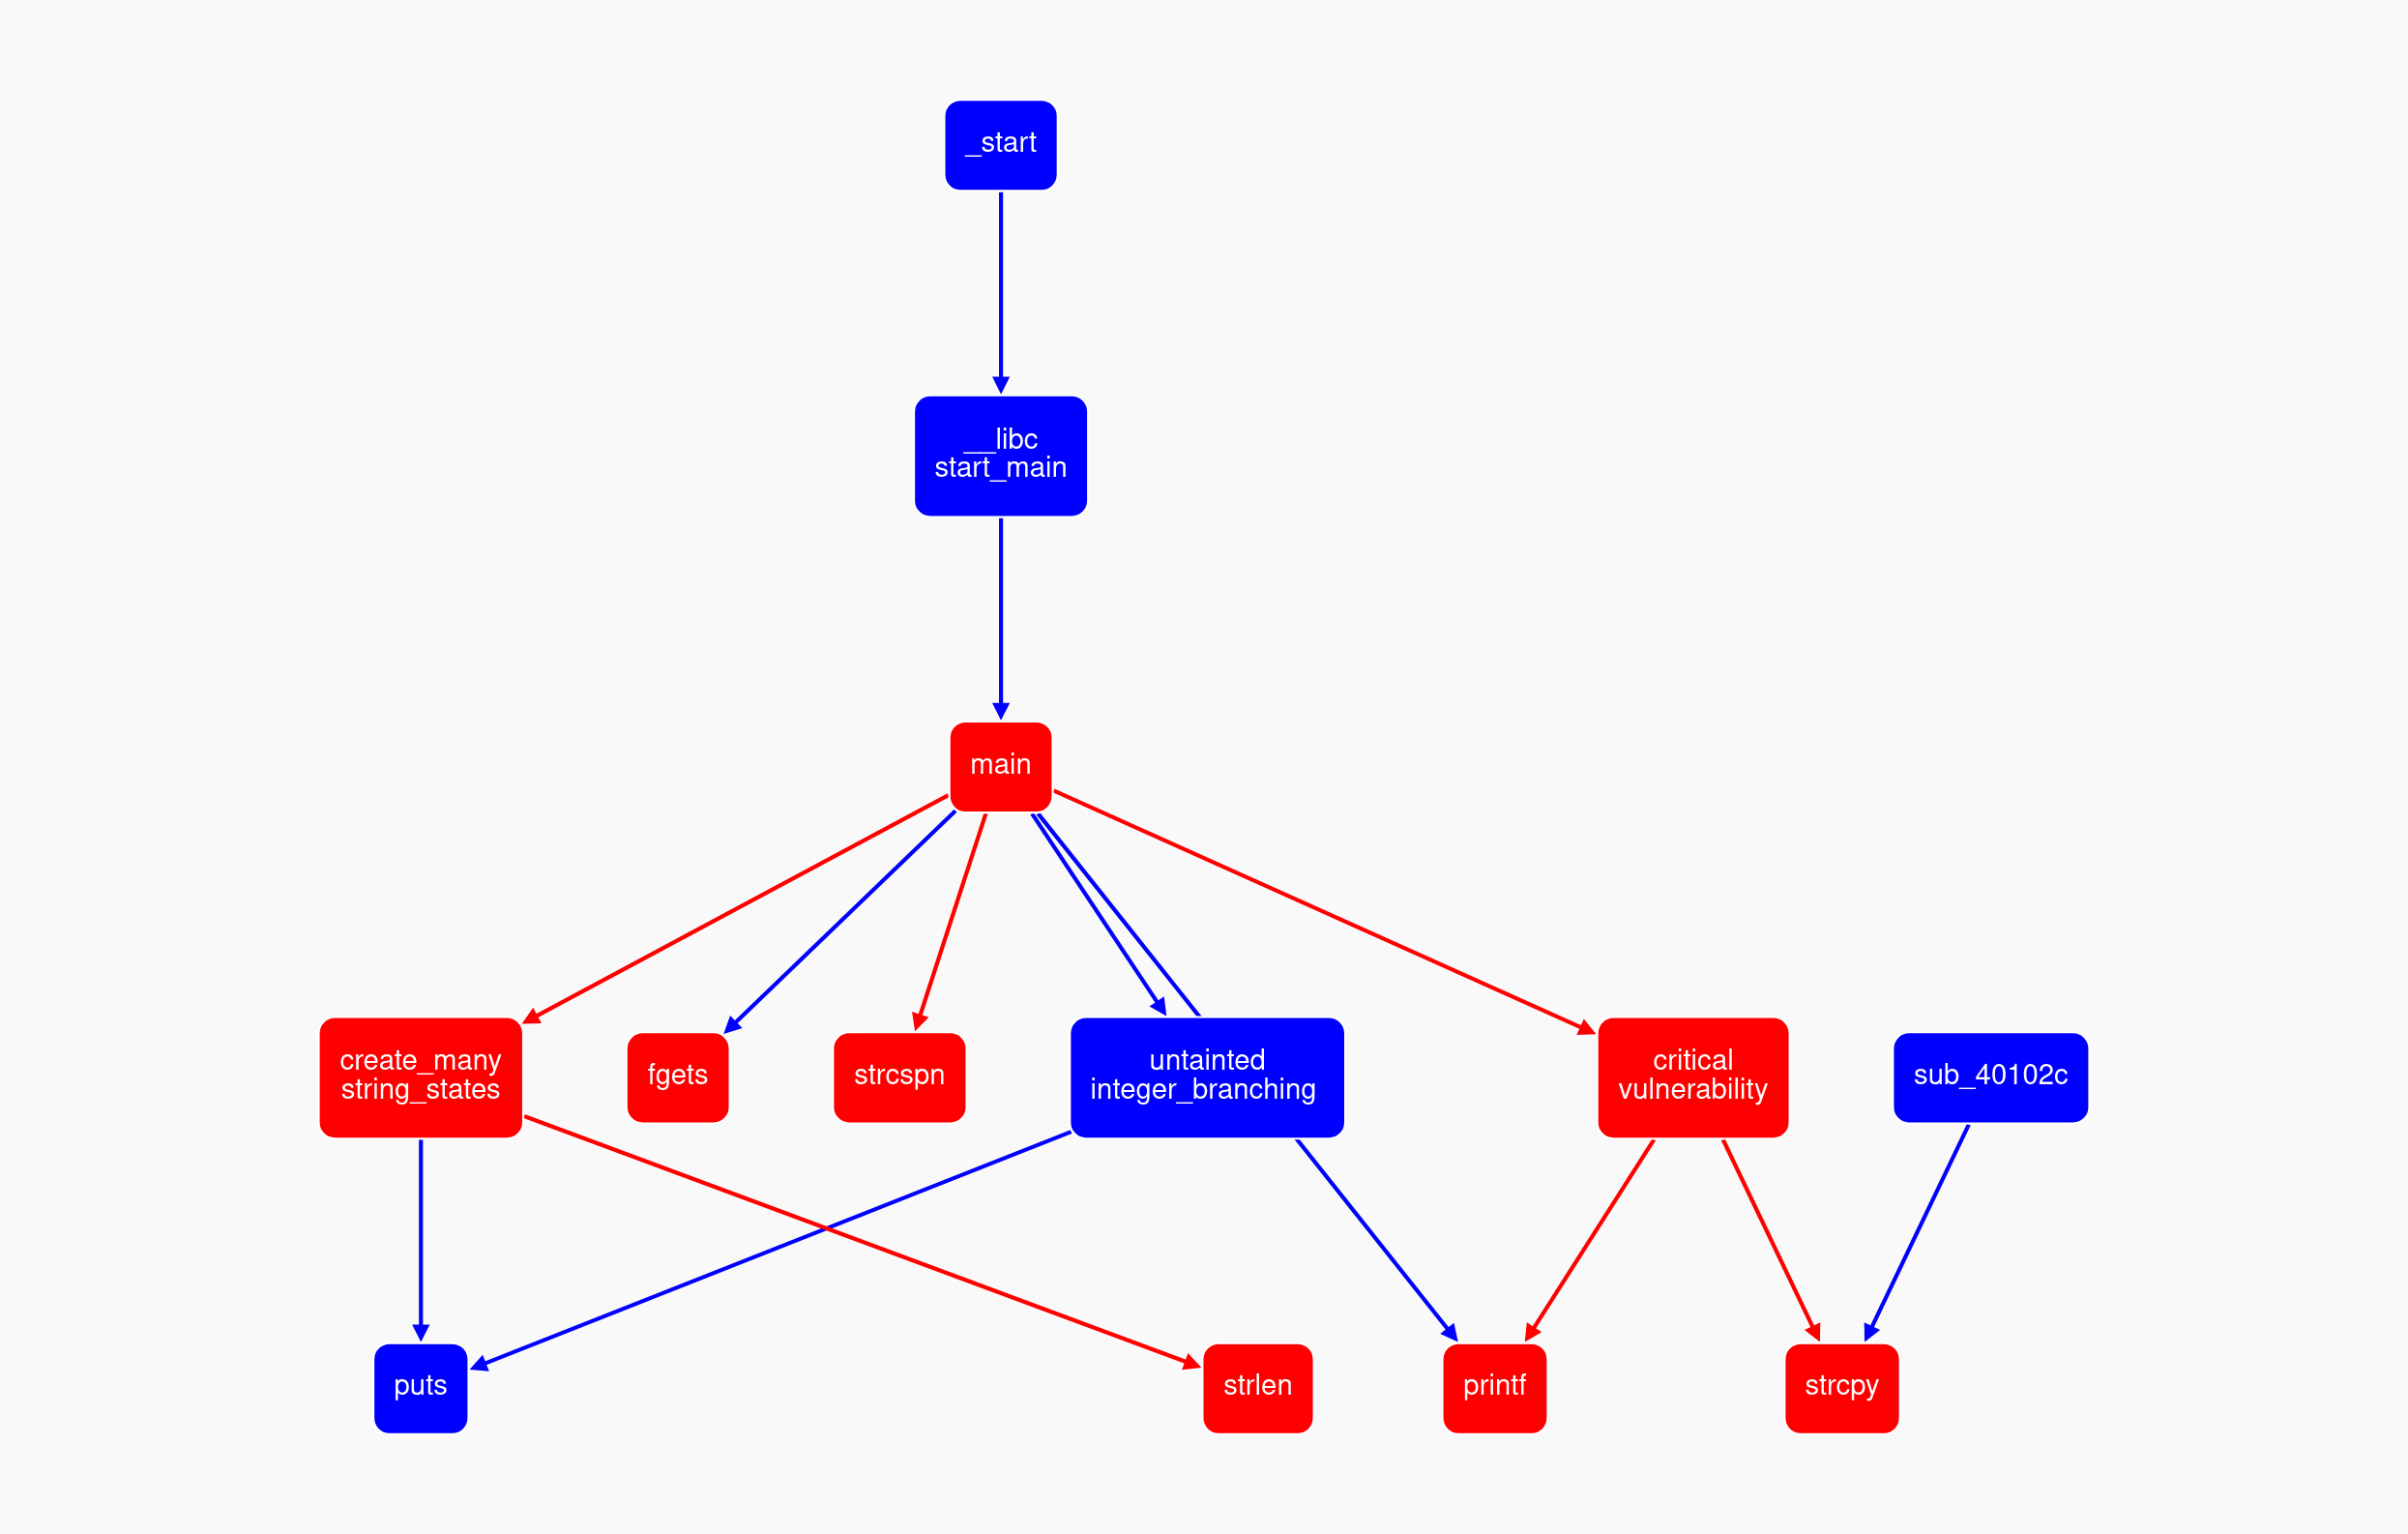
\includegraphics[width=0.9\textwidth]{Figures/test_state_explosion_visualization.png}
    \caption{Interactive visualization of taint flow analysis showing function call graph with taint propagation patterns. Red nodes and edges indicate tainted functions and data flow; blue elements represent untainted program regions.}
    \label{fig:test_state_explosion_visualization}
\end{figure}

Figure~\ref{fig:test_state_explosion_visualization} illustrates the call graph with clear distinction between security-relevant and irrelevant program regions. Red nodes represent functions processing tainted data, while red edges indicate tainted data flow between functions. Blue elements show untainted program regions that TraceGuard appropriately deprioritizes during exploration.
